% XJTLU Poster Template
% GitHub: https://github.com/yaoshanliang/XJTLU-Poster-Template

% Thanks to 
% https://www.overleaf.com/latex/templates/uq-poster-theme/nnhbtfwpjxpw
% https://github.com/alfurka/gemini-uq
% https://rev.cs.uchicago.edu/k4rtik/gemini-uccs
% https://github.com/anishathalye/gemini

\documentclass[final]{beamer}
% ====================
% Packages
% ====================
\usepackage[T1]{fontenc}
\usepackage{lmodern}
\usepackage[orientation=portrait,size=a0,scale=1.0]{beamerposter} % Current dimensions A0, put in your poster dimensions
\usetheme{gemini}
\usecolortheme{uchicago}
\usepackage{graphicx}
\usepackage{caption}
\usepackage{booktabs}
\usepackage{tikz}
\usepackage{pgfplots}
\pgfplotsset{compat=1.17}
\newcommand{\blu}{\color{blue}}
\usepackage{DejaVuSans}

\usepackage[caption=false,font=small,labelfont=sf,textfont=sf]{subfig}
\DeclareSubrefFormat{myparens}{#1(#2)}
\captionsetup[subfloat]{subrefformat=myparens}

%%%%%%%%%%%%%%%%%%%%%%%%%%%%%%%%%%%%%%%%%%%%%%%%%%%%%%%%%%%%%%%%%%%%%%%%%%%%%%
% Column environment setup
%%%%%%%%%%%%%%%%%%%%%%%%%%%%%%%%%%%%%%%%%%%%%%%%%%%%%%%%%%%%%%%%%%%%%%%%%%%%%%
% If you have N columns, choose \sepwidth and \colwidth such that
% (N+1)*\sepwidth + N*\colwidth = \paperwidth
% Follow structure to create difference column environments. 
\newlength{\sepwidthA} % Seperation distance between comulumns type A
\newlength{\colwidthA} % collumn width type A
\setlength{\sepwidthA}{0.25\paperwidth}
\setlength{\colwidthA}{0.5\paperwidth}

\newcommand{\separatorcolumnA}{\begin{column}{\sepwidthA}\end{column}}

% Second column environment. 
\newlength{\sepwidthB}
\newlength{\colwidthB}
\setlength{\sepwidthB}{0.0266\paperwidth}
\setlength{\colwidthB}{0.44\paperwidth}

\newcommand{\separatorcolumnB}{\begin{column}{\sepwidthB}\end{column}}

% You can also use these column commands to create columns inside columns and for creating new column formatting. 
% You can also have non even columns by creating more column environments or specifying the width when beginning a column environment. 
%%%%%%%%%%%%%%%%%%%%%%%%%%%%%%%%%%%%%%%%%%%%%%%%%%%%%%%%%%%%%%%%%%%%%%%%%%%%%%
% Title
%%%%%%%%%%%%%%%%%%%%%%%%%%%%%%%%%%%%%%%%%%%%%%%%%%%%%%%%%%%%%%%%%%%%%%%%%%%%%%

\title{WaterScenes: A Multi-Task 4D Radar-Camera Fusion Dataset and Benchmark on Water Surfaces}
\author{Authors: Author1, Author2, Author3 ~\\ Supervisors: Supervisor1, Supervisor2}
% \supervisor{Supervisors: Supervisor1, Supervisor2}
\institute[shortinst]{ Xi'an Jiaotong-Liverpool University}

%%%%%%%%%%%%%%%%%%%%%%%%%%%%%%%%%%%%%%%%%%%%%%%%%%%%%%%%%%%%%%%%%%%%%%%%%%%%%%
% Poster footer
%%%%%%%%%%%%%%%%%%%%%%%%%%%%%%%%%%%%%%%%%%%%%%%%%%%%%%%%%%%%%%%%%%%%%%%%%%%%%%

\footercontent{
\href{mailto:Author@xjtlu.edu.cn}{Author@xjtlu.edu.cn} % this is a clickable link
  \hfill
  Conference Name \hfill
  {Poster Number: \#} }
% (can be left out to remove footer)  

\begin{document}
%%%%%%%%%%%%%%%%%%%%%%%%%%%%%%%%%%%%%%%%%%%%%%%%%%%%%%%%%%%%%%%%%%%%%%%%%%%%%%
% Logo placements (optional)
%%%%%%%%%%%%%%%%%%%%%%%%%%%%%%%%%%%%%%%%%%%%%%%%%%%%%%%%%%%%%%%%%%%%%%%%%%%%%%
% \addtobeamertemplate{headline}{}
% {
%     %\begin{tikzpicture}[remember picture,overlay] % Solid header bar
%     \begin{tikzpicture}[remember picture,overlay,line width=\arrayrulewidth] % gradient header bar
%       % Logo 
%       \node [anchor=north west, inner sep=3cm] at ([xshift=0cm,yshift=1.0cm]current page.north west)
%       {\includegraphics[height=6.0cm]{logos/UQlockup-Reverse-cmyk.eps}}; 
%       % Logo 1, replace with custom logo
%       \node [anchor=north east, inner sep=3cm] at ([xshift=0.0cm,yshift=2.0cm]current page.north east)
%       {\includegraphics[height=8.0cm]{logos/Logo-Right.png}}; 
%       % Extra logo 2
%       \node [anchor=north east, inner sep=3cm] at ([xshift=1.0cm,yshift=-10.0cm]current page.north east)
%       {\includegraphics[height=6.0cm]{logos/UQlockup-Purple-cmyk.eps}};
%       %  Extra logo 3, or a QR Code
%       \node [anchor=north west, inner sep=3cm] at ([xshift=-1.0cm,yshift=-10.0cm]current page.north west)
%       {\includegraphics[height=7.0cm]{Figures/ChristopherGBaker_URL.eps}}; 
%     \end{tikzpicture}
% }

% ====================
% Body
% ====================

\begin{frame}[t]
%%%%%%%%%%%%%%%%%%%%%%%%%%%%%%%%%%%%%%%%%%%
%Section 1
%%%%%%%%%%%%%%%%%%%%%%%%%%%%%%%%%%%%%%%%%%%
\begin{columns}[t]
\begin{column}{0.53\paperwidth}
\begin{block}{\Large{\textbf{Abstract}}}
\large
\textcolor{purple}{\textbf{Autonomous driving on water surfaces}} plays an essential role in executing hazardous and time-consuming missions, such as maritime surveillance, survivors rescue, environmental monitoring, hydrography mapping and waste cleaning. 
This work presents WaterScenes, \textcolor{purple}{\textbf{the first multi-task 4D radar-camera fusion dataset}} for autonomous driving on water surfaces. Equipped with a 4D radar and a monocular camera, our Unmanned Surface Vehicle (USV) proffers \textcolor{purple}{\textbf{all-weather solutions for discerning object-related information}}. In addition to basic perception tasks, such as object detection, instance segmentation and semantic segmentation, we also provide annotations for free-space segmentation and waterline segmentation.
Leveraging the \textcolor{purple}{\textbf{multi-task and multi-modal data}}, we demonstrate that \textcolor{purple}{\textbf{4D radar-camera fusion can considerably improve the accuracy and robustness}} of perception on water surfaces, especially in adverse lighting and weather conditions.
WaterScenes dataset is public on \textcolor{purple}{\textbf{\url{https://waterscenes.github.io}}}.
\end{block}
\end{column}
\begin{column}{0.39\paperwidth}
\vspace{2cm}
\begin{figure}
\centering
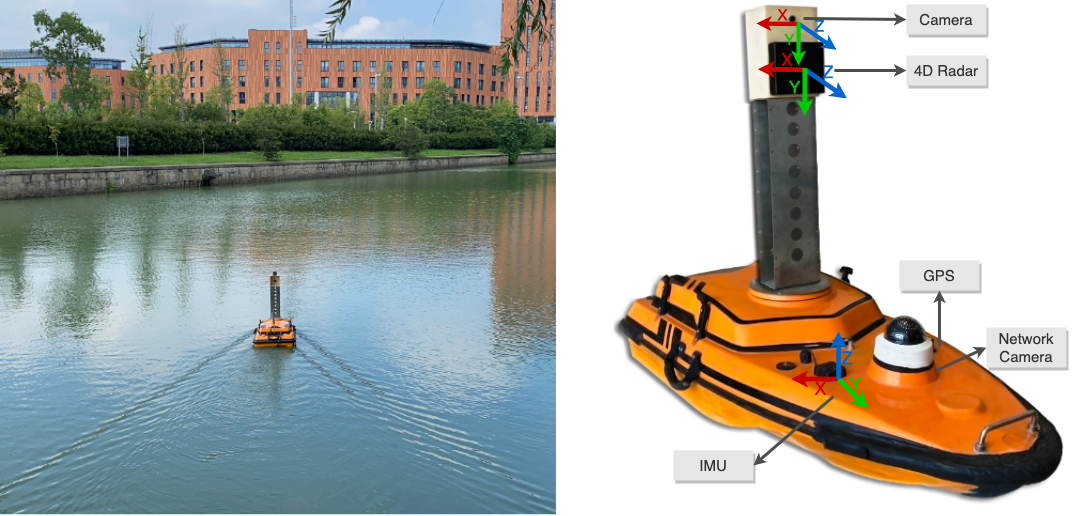
\includegraphics[width=1\textwidth]{images/usv.png}
\caption{Sensor suite for our USV and coordinate system of each sensor.}
\end{figure}
\end{column}
\end{columns}

%%%%%%%%%%%%%%%%%%%%%%%%%%%%%%%%%%%%%%%%%%%
%Section 2 
%%%%%%%%%%%%%%%%%%%%%%%%%%%%%%%%%%%%%%%%%%%
\begin{columns}
%%%%%%%%%%%%%%%%%%%%%%%%%%%%%%%%%%%%%%%%%%%
%Section 2 column 1
%%%%%%%%%%%%%%%%%%%%%%%%%%%%%%%%%%%%%%%%%%%
\separatorcolumnB
\begin{column}[T]{\colwidthB}
\begin{block}{\Large{\textbf{Contributions}}}
\vspace{0.5cm}
\large
$\Rightarrow$ We present WaterScenes, the first multi-task 4D radar-camera fusion dataset on water surfaces, which offers \textbf{data from multiple sensors, including a 4D radar, monocular camera, GPS, and IMU}. It can be applied in \textbf{six perception tasks, including object detection, instance segmentation, semantic segmentation, free-space segmentation, waterline segmentation, and panoptic perception}.

$\Rightarrow$ Our dataset covers \textbf{diverse time conditions} (daytime, nightfall, night), \textbf{lighting conditions} (normal, dim, strong), \textbf{weather conditions} (sunny, overcast, rainy, snowy) and \textbf{waterway conditions} (river, lake, canal, moat). 

$\Rightarrow$ We provide \textbf{2D box-level and pixel-level annotations for camera images, and 3D point-level annotations for radar point clouds}. We also offer a \textbf{toolkit} for WaterScenes that includes: pre-processing, labeling, projection and visualization, assisting researchers in processing and analyzing our dataset.

$\Rightarrow$ We build corresponding benchmarks and evaluate popular algorithms for object detection, point cloud segmentation, image segmentation, and panoptic perception. Experiments demonstrate the \textbf{advantages of radar perception on water surfaces, particularly in adverse lighting and weather conditions}.
\end{block}
    
\begin{block}{\Large{\textbf{WaterScenes Dataset}}}
\vspace{1cm}
\begin{figure}
\centering
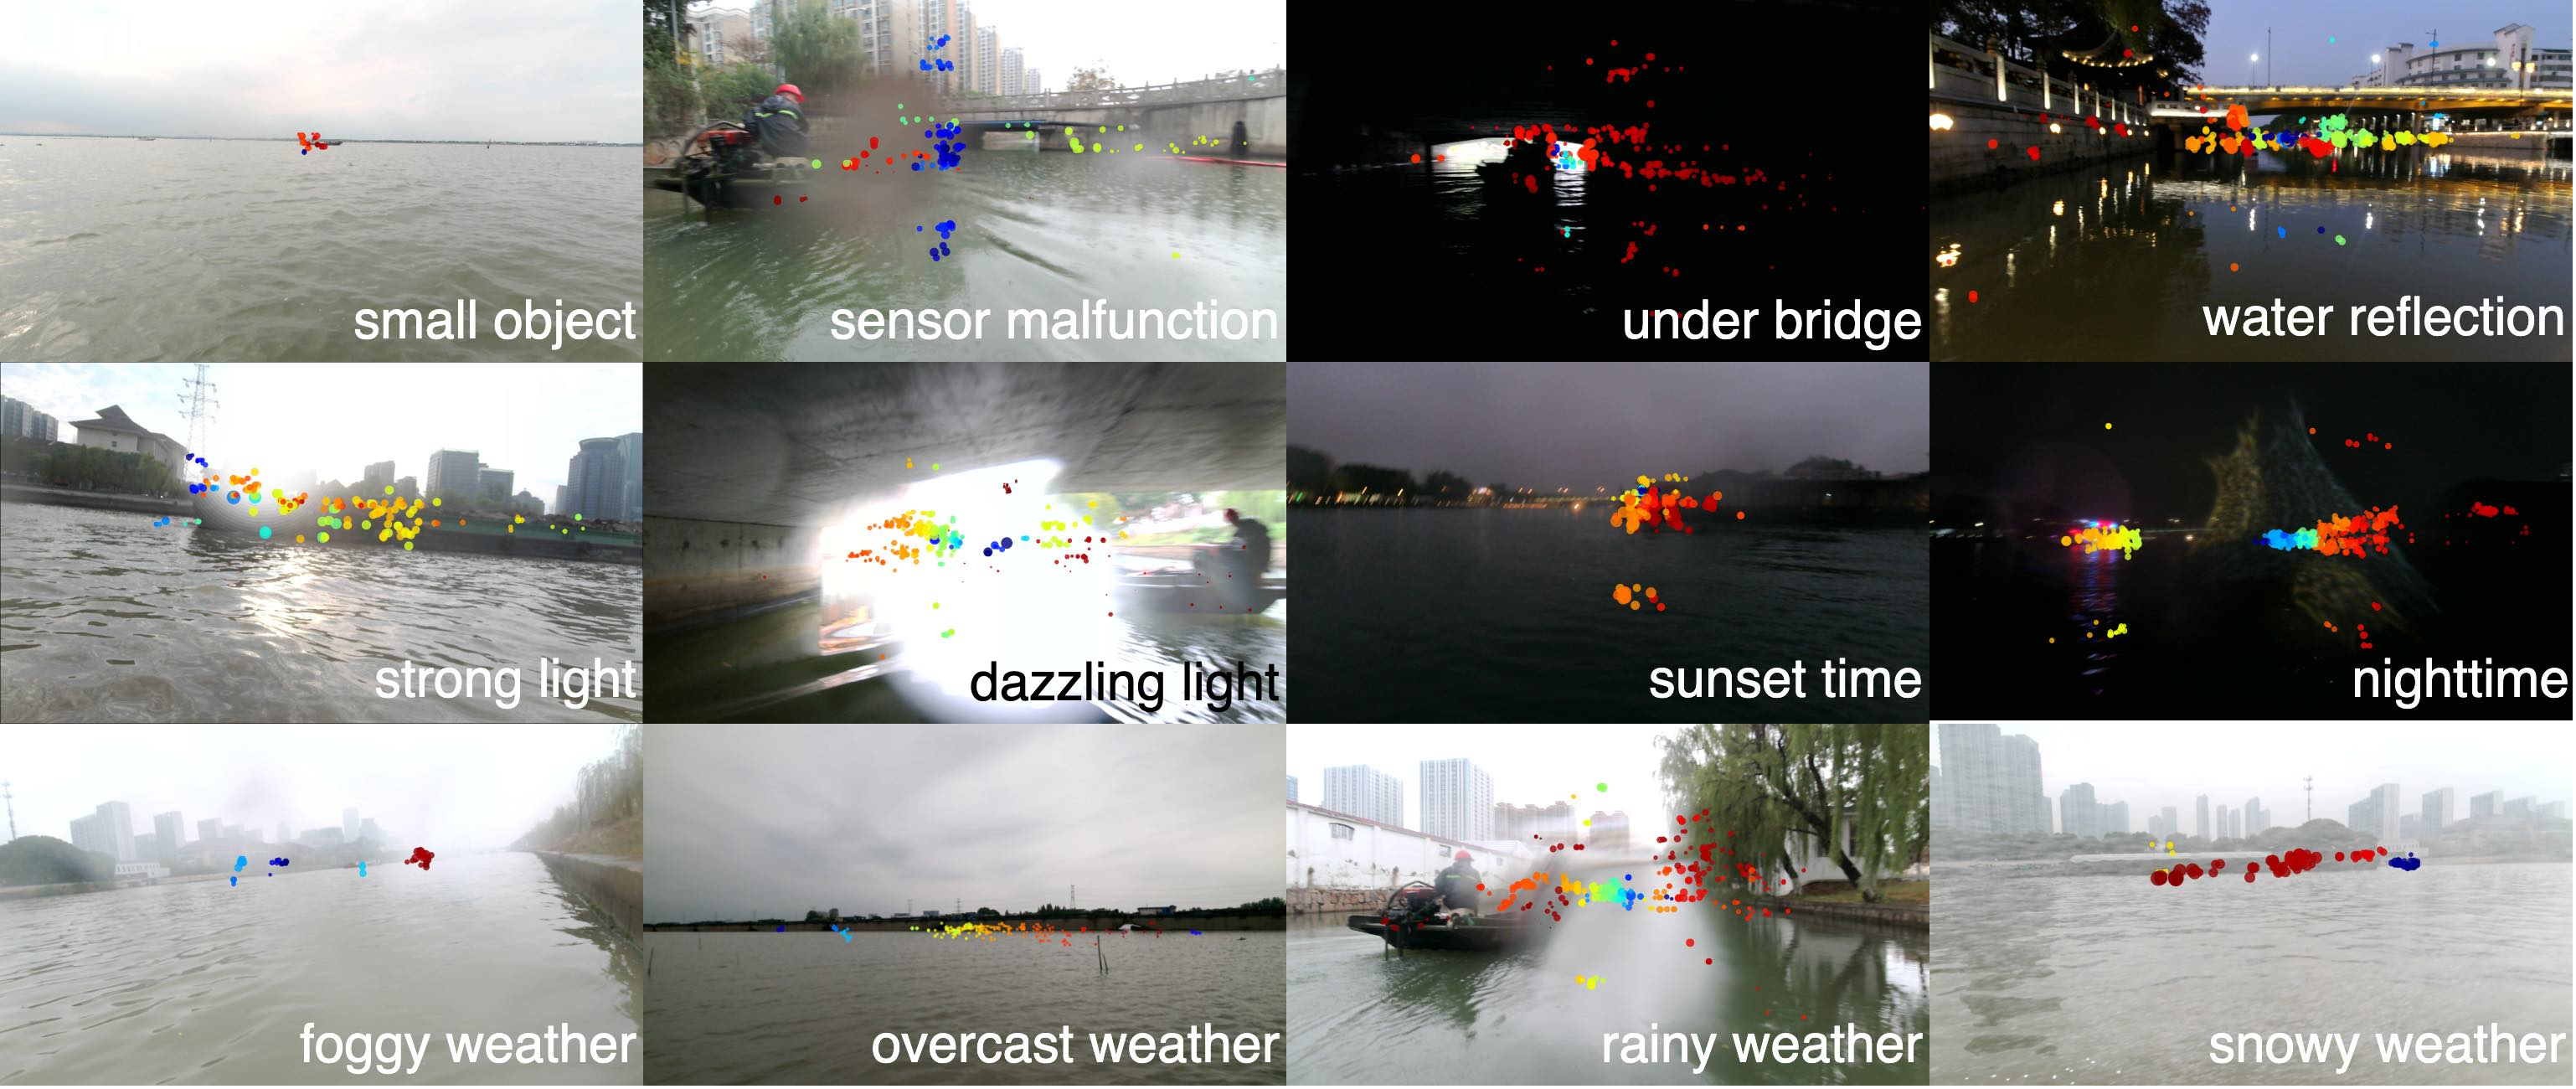
\includegraphics[width=1\textwidth]{images/samples}
\caption{Sample images in WaterScenes. Radar points are projected onto the image plane as colored dots.}
\end{figure}
\vspace{-1cm}

\begin{figure}[h]
\centering
\subfloat[Size distribution]{
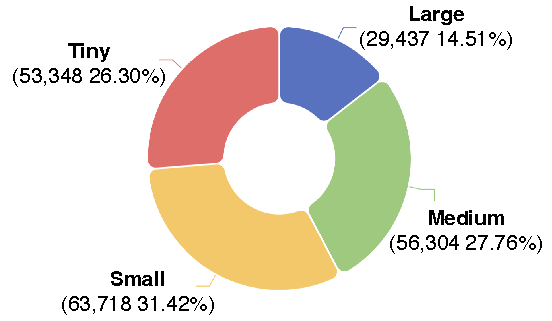
\includegraphics[width=0.47\columnwidth]{images/size}
\label{fig:size}
}
\quad
\hspace{-6mm}
\subfloat[Distance distribution]{
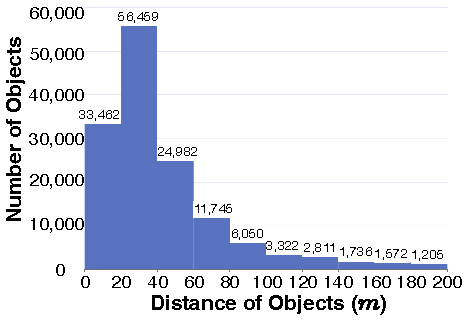
\includegraphics[width=0.43\columnwidth]{images/distance}
\label{fig:distance}
}
\caption{Statistics of objects in WaterScenes. (a) Wide range of object size. (b) Wide distribution of object distance.}
\label{fig:statistics}
\end{figure}

\vspace{-0.2cm}

\begin{table}[!h]
\caption{Statistics of each category in WaterScenes.}
\vspace{-0.8cm}
\normalsize
\setlength\tabcolsep{9pt}
\begin{tabular}{c|cccccccc}
\toprule
\bf{Category} & \bf{Pier} & \bf{Buoy} & \bf{Sailor} & \bf{Ship} & \bf{Boat} & \bf{Vessel} & \bf{Kayak} & \bf{Total} \\\midrule
Frames & 25,787 & 3,769 & 3,613 & 19,776 & 9,106 & 9,362 & 366 & 54,120 \\
Objects & 121,827 & 16,538 & 8,036 & 34,121 & 10,819 & 11,092 & 374 & 202,807 \\
Percentage & 60.07\% & 8.15\% & 3.96\% & 16.82\% & 5.33\% & 5.47\% & 0.18\% & 100\% \\\midrule
Points & 8.45 & 14.53 & 4.75 & 81.23 & 38.51 & 80.32 & 6.72 & 33.50\\
Power ($dB$)& 13.68 & 17.88 & 12.15 & 14.40 & 14.14 & 13.52 & 10.12 & 13.70 \\
Velocity ($m/s$) & 0.08 & 0.09 & 0.79 & 1.08 & 0.40 & 2.21 & 0.88 & 0.79\\
\bottomrule
\end{tabular}
\end{table}
\end{block}
\end{column}
\separatorcolumnB
%%%%%%%%%%%%%%%%%%%%%%%%%%%%%%%%%%%%%%%%%%%
%Section 2 column 2
%%%%%%%%%%%%%%%%%%%%%%%%%%%%%%%%%%%%%%%%%%%
\begin{column}[T]{\colwidthB}

   \begin{block}{\Large{\textbf{4D Radar-Camera Fusion Benchmark}}}
\vspace{0.5cm}
\large
We evaluate SOTA models on WaterScenes dataset. 
For object detection, we utilize YOLOv8 for camera-based detection and an early fusion method based on YOLOv8 modules for fusion-based detection. 
The evaluation results highlight the effectiveness of 4D radar-camera fusion for improving object detection accuracy, particularly in adverse lighting and weather conditions. 

% \large $\Rightarrow$ \textbf{\color{purple}{Detection}} 

\begin{figure}
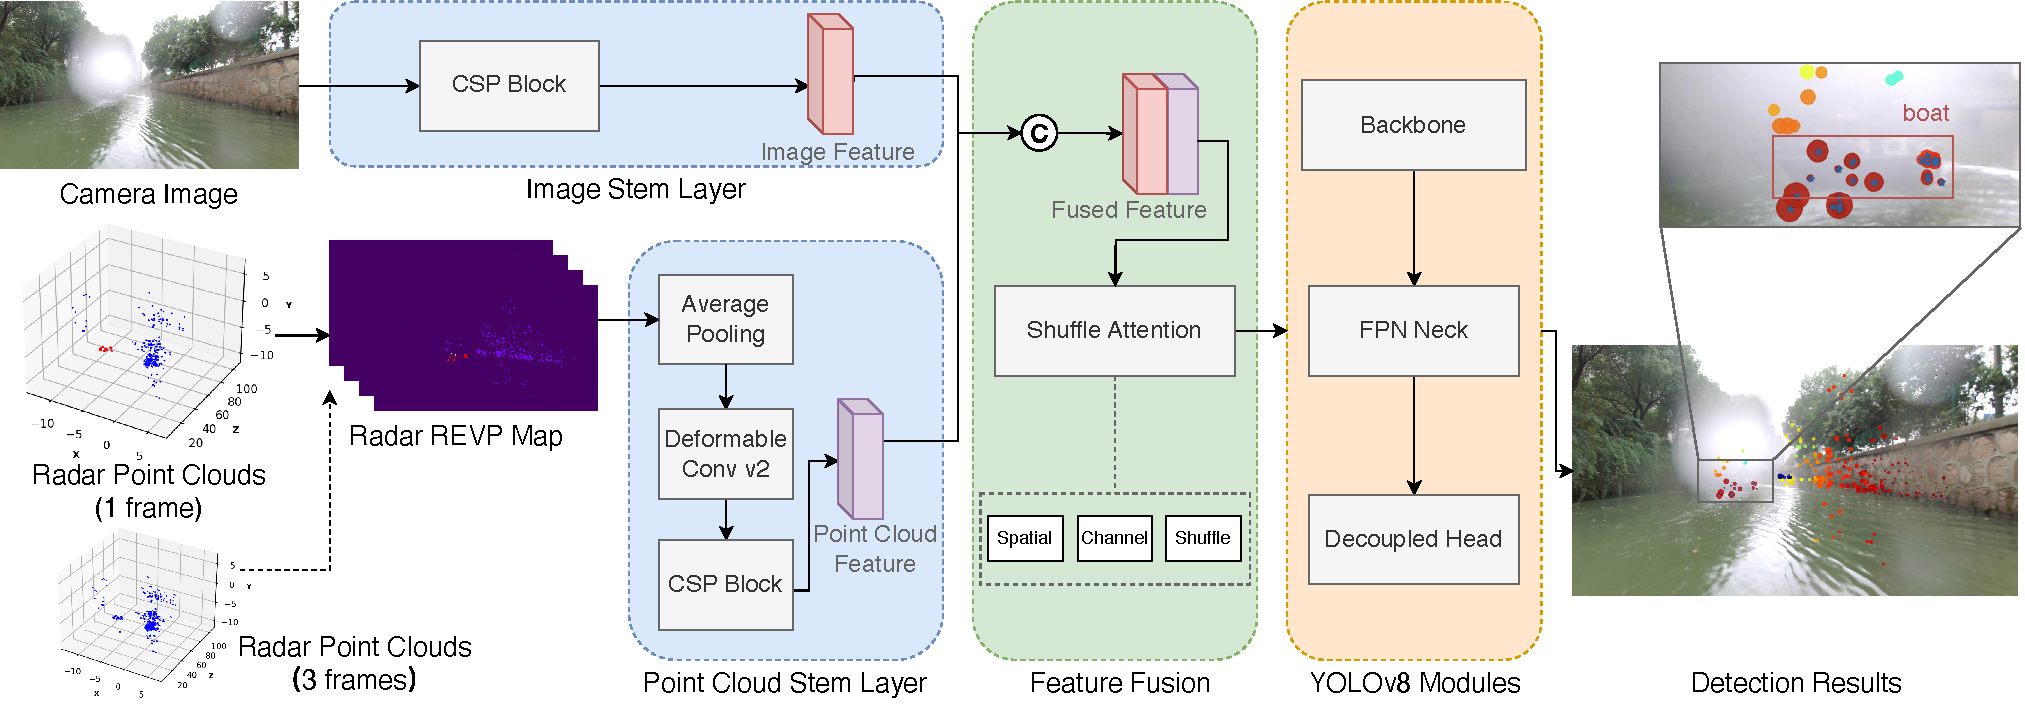
\includegraphics[width=1\textwidth]{images/network.pdf}
\caption{Radar-camera fusion network for the detection benchmark on WaterScenes dataset. Camera images and radar point clouds are fed into the stem layers for feature extraction. Subsequently, the extracted features are concatenated along the channel dimension and processed by the attention mechanism before forwarding into YOLOv8-M modules. As a result, the fusion-based network successfully detects the boat in scenarios where the camera is occluded by waterdrops.}
\end{figure}

\vspace{-0.7cm}
\begin{table}[!h]
\caption{Comparison of object detection performance using camera-based and fusion-based methods. In the Modalities column, C denotes the modality from the camera sensor, R denotes the modality from the 4D radar sensor, n-$\textup{frame(s)}$ denotes the accumulation of n-frame radar point clouds.}
\vspace{-0.5cm}
\setlength\tabcolsep{21pt}
\large
\begin{tabular}{c|ccc}
\toprule
\bf{Modalities} & \bf{mAP $_{@50}$} & \bf{Adverse Lighting} & \bf{Adverse Weather}\\\midrule
C & 84.4 & 74.9 & 79.5\\
C + R$_{1\mbox{-}\textup{frame}}$ & 88.0 (3.6$\color{purple}{\uparrow}$) & 80.1 (5.2$\color{purple}{\uparrow}$) & 82.4 (2.9$\color{purple}{\uparrow}$)\\
C + R$_{3\mbox{-}\textup{frames}}$ & 88.8 (4.4$\color{purple}{\uparrow}$) & 82.1 (7.2$\color{purple}{\uparrow}$) & 84.2 (4.7$\color{purple}{\uparrow}$)\\
\bottomrule
\end{tabular}
\end{table}

\begin{figure}[htbp]
\centering
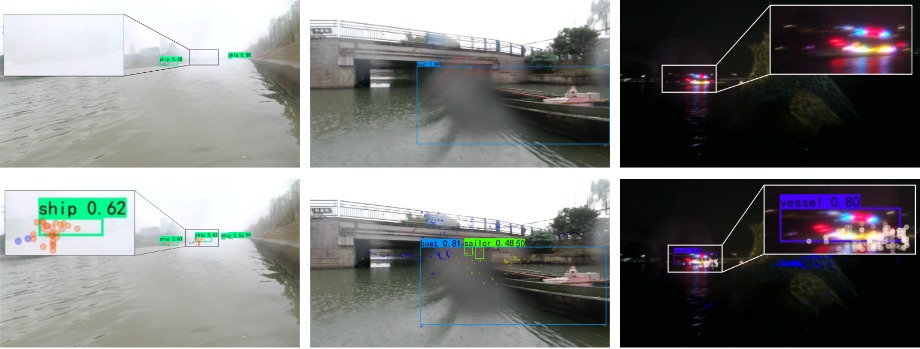
\includegraphics[width=0.95\columnwidth]{images/visualization}
\caption{Visualization of object detection results on WaterScenes. The first and second rows present camera-based YOLOv8-M and fusion-based YOLOv8-M, respectively.}
\end{figure}
\end{block}

\vspace{-0.5cm}
\begin{block}{\Large{\textbf{Conclusion}}}
\vspace{0.9cm}
\large
This work proposed a novel 4D radar-camera dataset named WaterScenes for six perception tasks on water surfaces. 
With the complementary advantages of radar and camera sensors, our dataset enables multi-attribute and all-weather perception of objects on water surfaces. 
Experimental results indicate that the 4D radar-camera combination is a robust solution for USVs on water surfaces. 
The presented WaterScenes offers a valuable resource for researchers interested in autonomous driving on water surfaces and aims to motivate novel ideas and directions for the development of water surface perception algorithms. 
\end{block}

\vspace{-0.5cm}
\begin{block}{\large{References}}
\vspace{0.5cm}
\normalsize
[1] Yao S, Guan R, Wu Z, et al. WaterScenes: A Multi-Task 4D Radar-Camera Fusion Dataset and Benchmark for Autonomous Driving on Water Surfaces[J]. arXiv preprint arXiv:2307.06505, 2023.
\end{block}

\end{column}
\separatorcolumnB
\end{columns}
\end{frame}
\end{document}
